% !TEX encoding = UTF-8 Unicode

\documentclass[twocolumn,10pt,a4j]{ltjsarticle}
\usepackage{kougai}
\usepackage{enumitem}
\usepackage{amsmath}
\renewcommand{\theenumi}{\textcircled{\arabic{enumi}}}

\title{アメリカザリガニによる水質の変化についてのシミュレーション}
\author{2132123 福田 勇太 2132129 堀田桃乃介  指導教員 須田 宇宙 准教授}
\date{}

\begin{document}

\maketitle

\section{はじめに}


%主な淡水魚は, 水草や藻類などの水草によって浄化された透き通った水環境に生息している.
%藻類は栄養素を吸収し水質を改善する一方で,過剰に繁殖すると水質悪化の要因となる.
%近年,生活排水による富栄養化や,外来種が水草などの水草を捕食することで起こる水質悪化により,淡水魚が生息しづらくなってきている.
%これにより,淡水魚の約25\%は絶滅の危機に陥っている\cite{env}.

現在,淡水魚の約25\%は絶滅の危機に陥っている.
その原因は,水質悪化・遺伝子汚染・乱獲・環境改変などと言われている.
そのうち水質悪化が高い割合を占めており,中でも生活排水や外来種によるものがある\cite{zetu}.
外来種の中でもアメリカザリガニの影響が大きいとされている\cite{env}.
アメリカザリガニの放流防止について,Web,本,学校での授業で啓発活動がされているが放流が減らないという問題がある.

これに対してアメリカザリガニが与える被害の大きさが具体的に分かれば放流が減り,水質悪化を抑えられることが期待できる.そこで本研究では,アメリカザリガニ・水草・水質の相互作用についてのシミュレーションを行うことを目的とする.

\section{アメリカザリガニによる影響}
アメリカザリガニは,底泥を巻き上げる行動や水草の切断・食害により,水質を悪化させている.
そのため現在は,条件付特定外来生物に指定されている.
通常,水域は栄養素が過剰にならないようにバランスが保たれているが,アメリカザリガニが侵入すると水草が減少し富栄養化になる.増えた栄養素を吸収し藻類が異常増殖して酸素が不足し,最終的に藻類が死滅した後に死骸が分解されず水質が悪化する.

%茨城県の宍塚大池の事例では,2020年ごろにアメリカザリガニが大量発生した.
%これにより,水草が著しく減少し,池の水が濁った.
% 原因としては,以下のような現象が生じたためである.\\
% ①図1(左)は水草が生い茂っており,栄養素が過剰にならないようにバランスを保っている\\
% ②アメリカザリガニにより水草が減少し,富栄養化になる\\
% ③藻類が栄養素を吸収し異常増殖する.\\
% ④酸素が不足し,藻類が死滅して水質が悪化し図1(右)のように水が濁る
% 現在,地域の協力によって1万匹以上のアメリカザリガニが駆除されているが,その繁殖力の強さから完全な駆除には至っていない

% \begin{figure}[h]
% \begin{center}
%   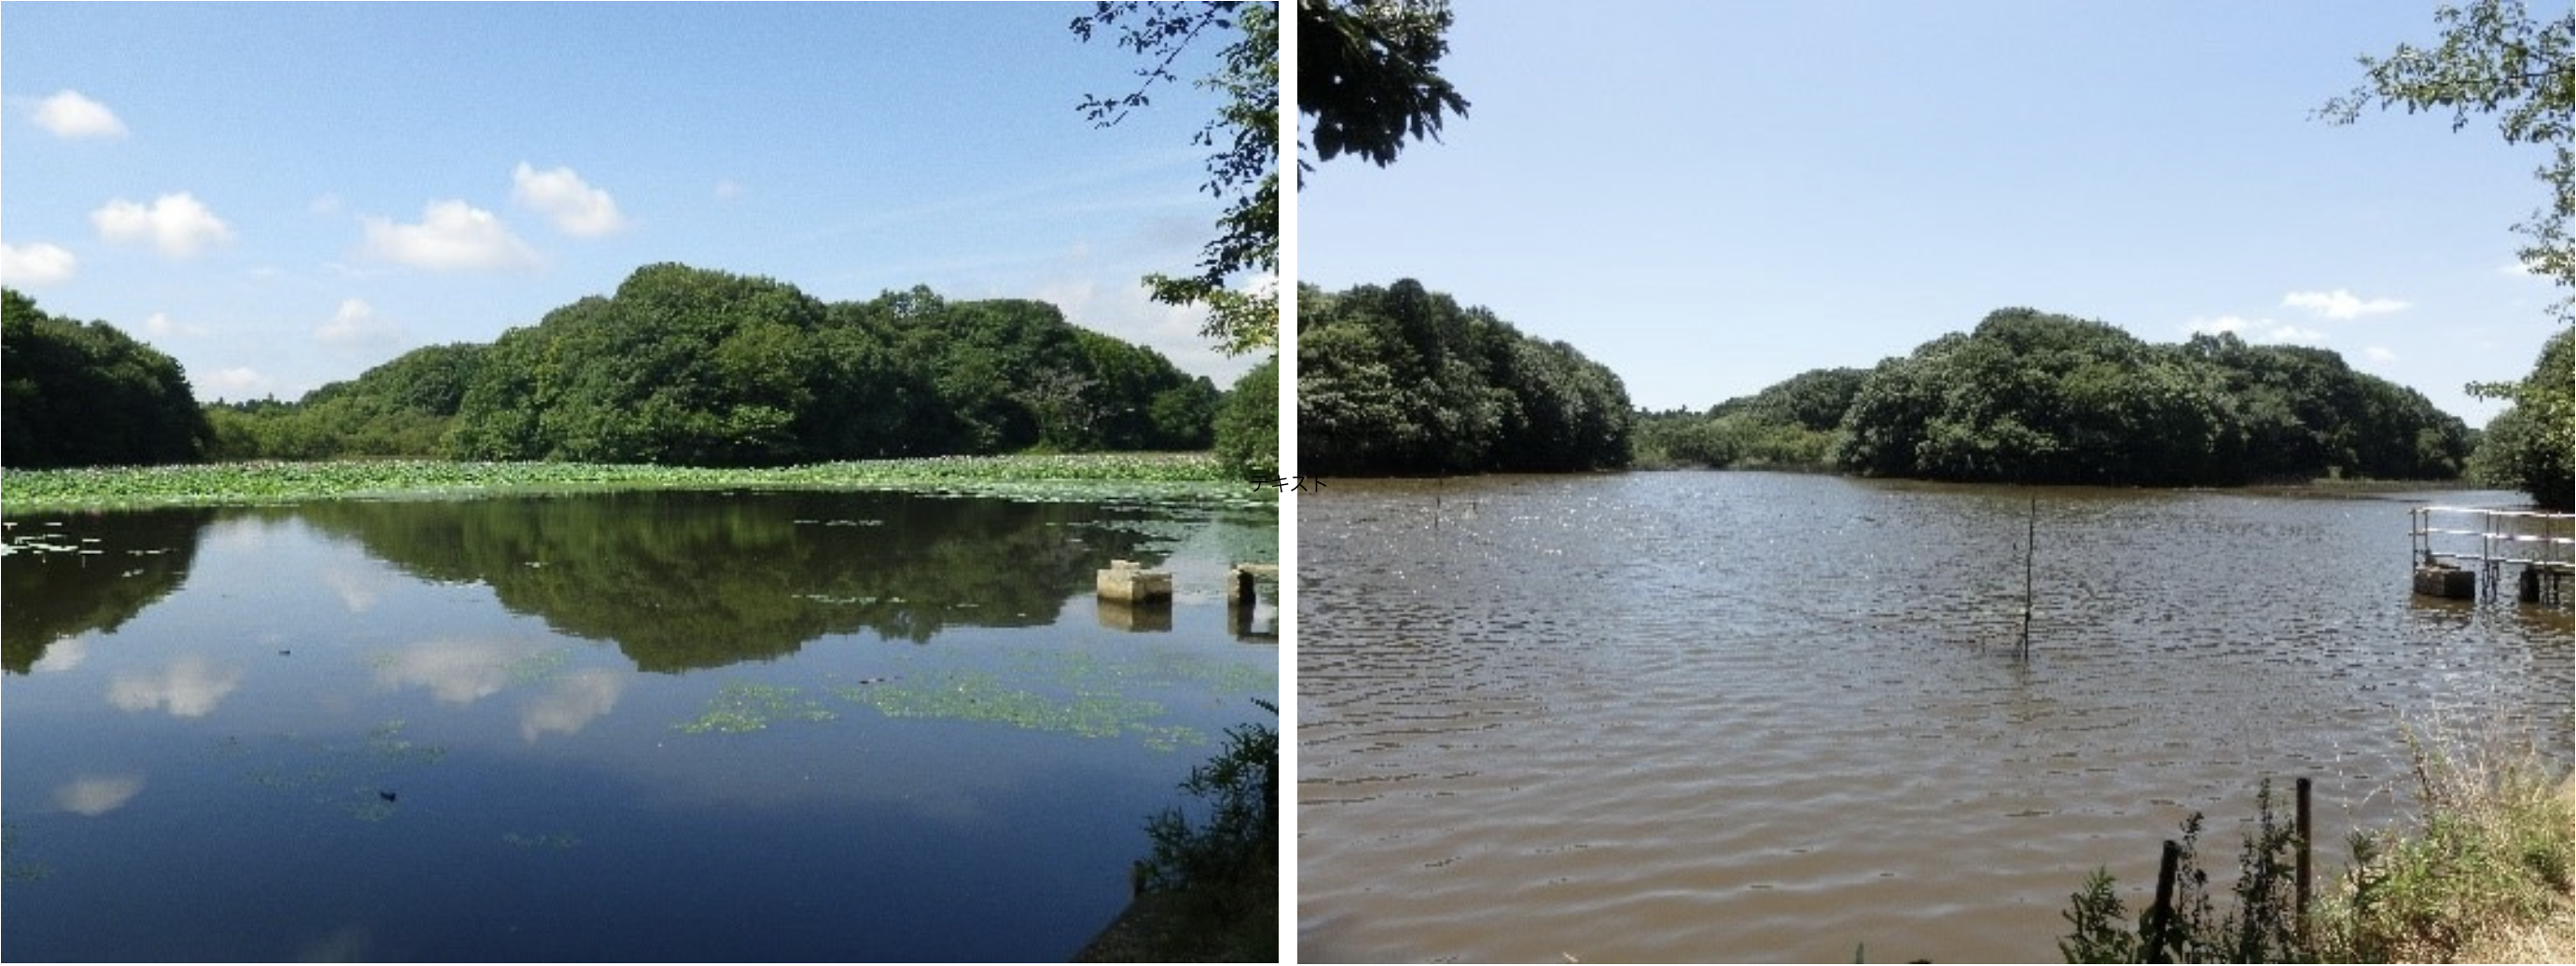
\includegraphics[width=.95\columnwidth]{新・水質.jpg}
% \end{center}
%   \caption{アメリカザリガニによる影響\\(左:侵入前,右:侵入後)}
%   \label{fig:切り替え}
% \end{figure}

\section{シミュレーションの概要}
本研究ではアメリカザリガニの繁殖における個体数の増加について生物の増加モデルであり,環境収容力という要素を組み込んだロジスティック方程式を利用する\cite{log}.
式\eqref{eq:one}に増加のモデルを示す.$N(t)は$その月における個体数,rは繁殖率,Eは環境収容力を表す.
\begin{equation}
  N(t+1) = N(t) + \mathrm{r} \cdot N(t) \cdot \left(1 - \frac{N(t)}{\mathrm{E}}\right)\label{eq:one}
\end{equation}
式\eqref{eq:one}をもとに作成した水草の減少モデルを式\eqref{eq:two}に示す.
$W(t)$はその月における水草の重さ,aは1匹のアメリカザリガニが1ヶ月で減少させる水草の重さである.
\begin{equation}
  W(t+1) = W(t) - a \cdot N(t)\label{eq:two}
\end{equation}

同様に,式\eqref{eq:one}をもとに作成した水質モデルを式\eqref{eq:three},\eqref{eq:four}に示す.
水質の指標は多数存在するが,本研究では濁りと藻類の濃度である,SS(Suspended Solids:懸濁汚染物質)とクロロフィルaを用いた.
$S(t)$,$C(t)$はその月におけるSS,クロロフィルaの重さ,
$k$,$h$は1匹のアメリカザリガニが1ヶ月で増加させるSS,クロロフィルaの重さ.
Lは水量を表す.

\begin{equation}
  S(t+1) = \frac{S(t) + k \cdot N(t)}{L}\label{eq:three}
\end{equation}

\begin{equation}
  C(t+1) = \frac{C(t) + h \cdot N(t)}{L}\label{eq:four}
\end{equation}

% 次に④について,C(t)はその月におけるクロロフィルaの量.h(μg)は過去に行われた実験データから取得したアメリカザリガニ1匹が1ヶ月で増加させるクロロフィルaの量である.N(t)はその月のアメリカザリガニの個体数である.そしてLはシミュレーションを行う池の水量である.

以上4つの式を使用しそれぞれの要素についてシミュレーションを行った.
図1の右軸はアメリカザリガニの個体数を表している.
左の縦軸は初期の水草の重さを100\%とする水草の割合を示している.
またSS濃度とクロロフィルa濃度に関する水草の基準値はそれぞれ$25\ \text{mg}/\text{L}$,$25\ \text{mg}/\text{L}$と定められておりこれを100\%とした.

\begin{figure}[h]
\begin{center}
  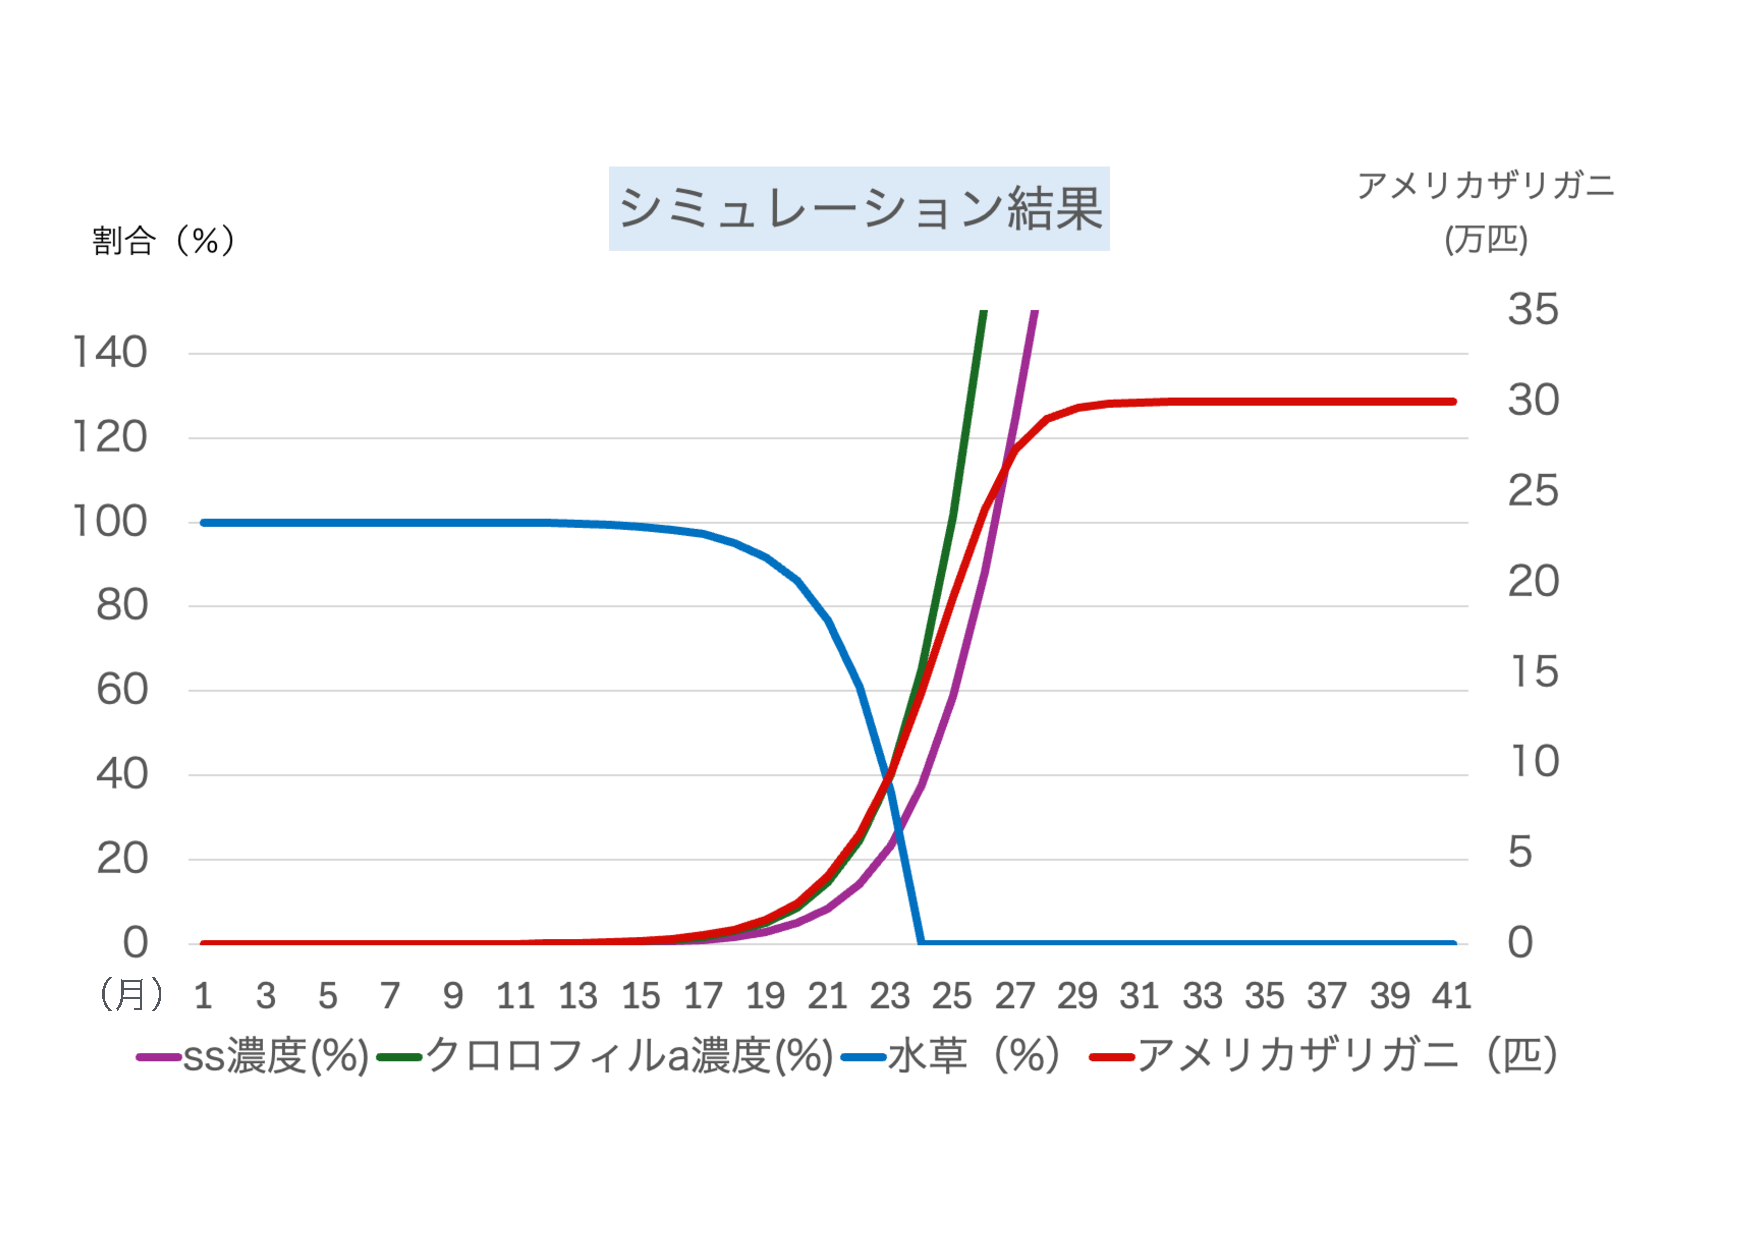
\includegraphics[width=.95\columnwidth]{graph6.pdf}
\end{center}
  \caption{シミュレーション結果\\}
  \label{fig:切り替え}
\end{figure}
図1から,アメリカザリガニの個体数の増加に伴って水草が大きく減少していることがわかった.
17,18ヶ月頃から環境が変わり始め,24カ月頃には壊滅的な環境になっていることがわかった.
また,水草の減少に伴ってSS濃度とクロロフィルa濃度が水質悪化の基準値を超えているということがわかった.


%本研究では, アメリカザリガニ・水草・水質の相互関係をモデル化しシミュレーションを行うことで, 少量のアメリカザリガニが生態系に与える悪影響を数値的に予測することを目指す.
%具体的には,以下のような生物や環境間の相互作用を過去の実験データから取得し模していく\cite{kasumigaura}.

%\begin{enumerate}
%  \item アメリカザリガニが水中の栄養素を吸収している水草を切断,または食べることで水草は減る
%  \item 水中の栄養素を吸収する水草が減り,富栄養化になる
%  \item 植物プランクトンや藻類が大量繁殖し,水面が緑色になるアオコを招く
%  \item 水中の溶存酸素が不足し, 植物プランクトンや藻類が死滅して水質が悪化する
%\end{enumerate}

%このように,アメリカザリガニは水草を減少させることで水質に悪影響を与えている.ここで,\textcircled{2}〜\textcircled{4}は\textcircled{1}による連鎖的な現象であり,水質の悪化としてまとめ,アメリカザリガニ・水草・水質の三要素からなるモデルとした.モデルの詳細には,実験を行った研究で得られている実験データも考慮する.

%以上のように,アメリカザリガニは水草の減少を通じて水質に大きな影響を与える.
%中でも,アメリカザリガニが及ぼす直接的な影響は①である.
%この影響が連鎖的に②〜④のように水質悪化の原因となる.

%このように,アメリカザリガニは水草を減少させることで水質に悪影響を与えている.
%ここでによる,\textcircled{2}〜\textcircled{4}は\textcircled{1}連鎖的な現象であり,水質の悪化としてまとめることができる.
%よって本研究では,アメリカザリガニ・水草・水質の相互関係をモデル化しシミュレーションを開発していく.


\section{おわりに}
今回,啓発活動において1,2匹あたりが及ぼす水質悪化の被害の大きさが示されていないため啓発活動の効果が薄く放流が減らないことが問題であった.それに対し,シミュレーションによって被害の大きさを示すことができた.特に,アメリカザリガニの急激な繁殖による水草の減少がわかった.
このことから,将来的に放流が減り水質悪化が抑えられることが期待できる.
%シミュレーションに使用する三要素の関係を過去に行われた実験データから取得し, 式を作成しグラフを作成する.

%このシミュレーションを通じて,少量のアメリカザリガニによる影響を数値的に予測することができれば,
%少量の放流が引き起こす問題がわかりやすくなる.その結果,生態系への影響が軽減し,水質悪化がより抑えられることが期待される.
\begin{thebibliography}{99}
% \bibitem{FreshWater}IUCN: ``Freshwater fish highlight escalating climate impacts on species - IUCN Red List | International Union for Conservation of Nature – United States'', 
% \url{https://iucnus.org/news/freshwater-fish-highlight-escalating-climate-impacts-on-species-iucn-red-list/}, (2024/09/01参照)
\bibitem{zetu}``世界の淡水魚の4分の1が絶滅の危機:気候変動の影響大きく-オルタナ'', 
\url{https://www.alterna.co.jp/108565/}, (2024/09/01参照)
\bibitem{env} 環境省: ``自然環境・生物多様性'', 
\url{https://www.env.go.jp/nature/amezari_keii.html}, (2024/09/01参照)

% \bibitem{nani} 環境省: ``何が問題なの? 水草、全部切る!?'', \url{https://www.env.go.jp/nature/amezari_mondai.html}, (2024/09/01参照)

\bibitem{log} Lotka AJ 1925 Elements of Physical Biology (Baltimore, MD Williams  Wilkins Co.)

% \bibitem{kasumigaura}Shin-ichiro S. Matsuzaki , Nisikawa Usio , Noriko Takamura , Izumi Washitani, “Contrasting impacts of invasive engineers on freshwater ecosystems: an experiment and meta-analysis”, Oecologia, vol. 158, pp. 673–686, 2009
%\bibitem{env count} 環境省: ``アメリカザリガニ対策の手続き'', 2023 , \url{https://www.env.go.jp/content/900503465.pdf},(2024-09-1).
%\bibitem{ishikawa} 石川県: ``アメリカザリガニ'', \url{https://www.pref.ishikawa.lg.jp/sizen/gairaishu/amerikazarigani.html}, (2024/10/10参照).
% \bibitem{seitaikei} 国立環境研究所: “気候変動と生物多様性について”, 2018\url{https://cger.nies.go.jp/cgernews/201810/334002.html}, (2024/10/2参照)
%\bibitem{biwako} 田上愛子, 久保洋昭, 加賀昭和, 近藤明 ,井上義雄, ``琵琶湖の流動と水質のシミュレーション'',生産研究 59, 1 (2007).

%\bibitem{nishijima2017} Nishijima, Nishikawa, Miyashita, ``Habitat modification by invasive crayfish can facilitate its growth through enhanced food accessibility'', BMC Ecol 17, 37 (2017).



\end{thebibliography}

\end{document}
